\documentclass[11pt,dvipdfmx]{article}

\usepackage{deauthor,times}%Compulsory packages

\usepackage{bmpsize}
% \RequirePackage[dvips]{graphicx}


% \graphicspath{{zick/}}

\usepackage{url}
\usepackage{wrapfig,booktabs,multirow}
% \usepackage[ruled,linesnumbered]{algorithm2e}
\usepackage{subcaption}
\usepackage{amsmath}
\usepackage{amsfonts,amssymb}
\usepackage{xspace}
\usepackage{tcolorbox}


\newcommand{\USW}{\mathtt{USW}}
\newcommand{\R}{\mathbb{R}}
\newcommand{\N}{\mathbb{N}}
\newcommand{\OPT}{\mathrm{OPT}}
\newcommand{\ASTC}{\textsc{AssignTC}\xspace}
\newcommand{\PoD}{\mathit{PoD}}
\newcommand{\tup}[1]{\langle #1 \rangle}
\newcommand{\poly}{\mathit{poly}}

\begin{document}

\title{Fairness and Diversity in Public Resource Allocation Problems\footnote{Parts of this article are published in AAMAS 2018 \cite{benabbou2017diversity} and accepted to IJCAI 2019 \cite{benabbou2019fairness}.}}

\author{Nawal Benabbou$^1$, Mithun Chakraborty$^2$, Yair Zick$^2$\\
	$^1$Sorbonne Universit\'e, CNRS, Laboratoire d'Informatique de Paris 6, LIP6 F-75005 Paris, France\\ 
	\texttt{nawal.benabbou@lip6.fr}\\
	$^2$Department of Computer Science, National University of Singapore, Singapore\\
	\texttt{\{mithun,zick\}@comp.nus.edu.sg}
}

\maketitle             

\begin{abstract}
In this article, we address important extensions to the problem of allocating indivisible items to a population of agents: The agents are partitioned into disjoint groups on the basis of attributes (e.g., ethnicity) and we want the overall utility of the allocation to respect some notion of \emph{diversity} and/or \emph{fairness} with respect to these groups. We study two specific incarnations of this general problem. First, we address a constrained optimization problem, inspired by diversity quotas in some real-world allocation problems, where the items are also partitioned into blocks and there is an upper bound on the number of items from each block that can be assigned to agents in each group. We theoretically analyze the price of diversity -- a measure of the overall welfare loss due to these capacity constraints -- and report experiments based on two real-world data sets (Singapore public housing and Chicago public school admissions) comparing this constrained optimization-based approach with a lottery mechanism with similar quotas. Next, instead of imposing hard constraints, we cast the problem as a variant of fair allocation of indivisible goods -- we treat each group of agents as a single entity receiving a bundle of items whose valuation is the maximum total utility of matching agents in that group to items in that bundle; we present algorithms that achieve a standard relaxation of envy-freeness in conjunction with specific efficiency criteria.
%\keywords{Fair Allocation of Indivisible Items  \and Typewise Envy-freeness up to one item \and Non-wasteful Allocation.}
\end{abstract}

\section{Introduction}\label{sec:intro}
Over the years, the Singapore government has adopted several social integration measures, to accommodate its multi-ethnic and multi-cultural population; one of these is the {\em Ethnic Integration Policy} (EIP) used by the Housing and Development Board (HDB) since 1989 \cite{Parl1989} to determine housing allocations. This government body is charged with the construction of government subsidized public housing estates, and selling them to Singapore residents. 
The EIP sets upper bounds on the percentage of flats in every estate that can be owned by households of every major ethnic group: since 5 March 2010, every HDB housing block is required to hold no more than $87\%$ Chinese, $25\%$ Malay, and $15\%$ Indian/Others \cite{HDB10PR,deng2013publichousing}. 
These ethnic quotas prevent the over-representation of any one group in an estate (resulting in de-facto segregation). 
HDB uses a lottery to allocate new developments: all applicants who apply for a particular development pick their flats in a random order. 
Under the lottery mechanism, applicants selected later in the order may not get their top choices; in fact, they may be rejected because the quota for their ethnic group has been filled, {\em even if there are empty flats that they are willing to take}.
\begin{example}
	Consider an estate with 100 flats; Amirah (who is ethnically Malay) receives a queue number of 30 --- i.e., she is the 30th person to choose a flat; if, by random chance, 25 ethnic Malays precede her in the queue and pick before her, the ethnic quota for Malays (25\%) will be filled and Amirah will no longer be allowed to select a flat in that estate. On the other hand, if Amirah is 110th in line but all families preceding her in the queue are ethnically Chinese, then at most 87 out of the 100 flats will be taken (since the Chinese have an 87\% quota) and Amirah will have at least 13 flats to choose from. \hfill $\blacklozenge$
\end{example}
Over $72\%$ of Singapore apartments are HDB flats~\cite{Sing2018}, housing an estimated $81\%$ of Singapore residents \cite{HDB18keystats} as of 2018; thus, the HDB public housing market has a significant impact on the life and welfare -- both individual and collective -- of this island nation \cite{chua1991race,deng2013publichousing,kim2013singapore,sim2003public,wong2014estimating}. 
The HDB lottery mechanism, coupled with ethnicity constraints, adds another layer of complexity to what is, at its core, similar to the classic weighted bipartite matching or \emph{assignment} problem \cite{kuhn1955hungarian,munkres1957algo}: agents (buyer households) have idiosyncratic values/utilities for items (flats) while a central planner (HDB) wishes to allocate at most one item to each agent and vice versa, with the economic criterion of \emph{overall utility/welfare/efficiency} in mind -- but also with an added social goal of \emph{promoting diversity}. 
Inspired by diversity-respecting allocation mechanisms --- prevalent not only in Singapore public housing but also in other domains such as matching residents to hospitals in Japan, school admissions in many U.S. cities, and more \cite{kamada2015efficient,USedu2017,fragiadakis2017improving} --- we formally study the balance between maximizing allocative welfare and promoting allocative diversity. This underlying problem of allocation/assignment of goods distinguishes our contribution from the extensive literature on fairness and diversity in subset selection (see e.g., \cite{stoyanovich2018online,bredereck2018multiwinner} and references therein). 

In Section~\ref{sec:assigntc}, we analyze a (simplified) HDB housing market as an extension to the assignment problem where the sets of agents and items are partitioned into subsets called \emph{types} and \emph{blocks} respectively; there is a pre-specified upper bound on the number of agents of each type that can be assigned items in each block, called \emph{type-block capacities}. 
We analyze the {\em price of diversity}, i.e., the fractional loss in the overall (optimal) welfare due to these capacity constraints, and relate it to a measure of \emph{type disparity}; we also report simulations based on recent, real-world data sets, comparing our constrained optimization approach with a lottery mechanism with ethnicity quotas in terms of welfare.     

In Section~\ref{sec:grfair}, we present an alternative approach towards the efficiency-diversity trade-off, drawing on and adding to the rich literature on the fair division of indivisible goods (see e.g., \cite{procaccia2014fair,caragiannis2016unreasonable,kurokawa2016can,barman2017finding,barman2017approx}). Here, each type is represented by a \emph{super-agent} that is allocated a \emph{bundle} of items; the super-agent's valuation of a bundle is given by the maximum utility assignment of items in the bundle to agents of that type. When agent-item utilities are binary, we provide a polynomial-time algorithm that computes an allocation with the maximum (utilitarian) social welfare while satisfying a popular fairness criterion: \emph{envy-freeness up to one item} (EF1) \cite{budish2011combinatorial}; for arbitrary real-valued utilities, we show experimentally that a heuristic extension of the classic \emph{envy-graph algorithm} due to Lipton et al. \cite{lipton2004approximately} produces an EF1 allocation with low \emph{waste} (a new inefficiency concept that we have introduced for this setting).

\section{Diversity through hard capacity constraints}\label{sec:assigntc}
First, let us rigorously formulate the welfare maximization problem in a bipartite matching setting under type-block capacity constraints. Detailed proofs of all theoretical results in this section can be found in Benabbou et al. \cite{benabbou2017diversity}. Throughout the paper, for $s \in \N$, we denote the set $\{1, 2,\ldots, s\}$ by $[s]$. 
\begin{definition}[\ASTC]\label{def:AwTC}
	An instance of the Assignment with Type Constraints (\ASTC) problem is given by: (i) a set $N$ of $n$ agents partitioned into $k$ types $N_1,\dots, N_k$, (ii) a set $M$ of $m$ items/goods partitioned into $l$ blocks $M_1,\dots,M_l$, (iv) a utility $u(i,j) \in \R_+$ for each agent $i \in N$ and each item $j \in M$, and (iv) a capacity $\lambda_{pq} \in \N$ for all $(p,q) \in [k]  \times [l]$; $\lambda_{pq}$ is an upper bound on the number of agents of type $N_p$ allowed in block $M_q$. W.l.o.g. we assume that for all $p,q$, $\lambda_{pq} \le |M_q|$.
\end{definition}
An assignment of items to agents, which we will also sometimes call an $(N,M)$-matching, can be represented by a $(0,1)$-matrix $X  =  (x_{ij})_{n \times m}$ where $x_{ij} = 1$ if and only if item $j$ is assigned to agent $i$.
Our objective is to maximize the utilitarian social welfare or $\USW$, i.e., the sum of agent utilities: $u(X) \triangleq \sum_{i \in N}\sum_{j \in M} x_{ij} u(i,j)$.
Clearly, this optimization problem can be formulated as an integer linear program (ILP) as in Figure~\ref{linprog}. Here, the first set of inequalities captures our \emph{type-block constraints} while the last three sets are the usual \emph{matching constraints} jointly ensuring that each item (resp. agent) is assigned to at most one agent (resp. item).
\begin{wrapfigure}[14]{O}[-15pt]{0.42\textwidth}
	\vspace{-20pt}
	\begin{center}
		$\boxed{\begin{aligned}
			\max  			& \sum_{i \in N}\sum_{j \in M} x_{ij} u(i,j) &\\
			\mathit{s.t.} & \sum_{i \in N_p} \sum_{j \in M_q} x_{ij} \le \lambda_{pq} & \forall p \in [k], \forall q \in [l]\\
			&   \sum_{j \in M} x_{ij} \le 1 & \forall i \in N\\
			& \sum_{i \in N}  x_{ij}  \le 1 & \forall j \in M \\
			& x_{ij} \in\{0,1\} & \forall i \in N, \forall j \in M
			\end{aligned}}$
		\caption{ILP formulation of \ASTC. \label{linprog}}
	\end{center}
\end{wrapfigure}
In general, the decision version of the \ASTC problem is NP-complete (Benabbou et al. \cite[Theorem 3.2]{benabbou2017diversity}) but admits a polynomial-time $\tfrac{1}{2}$-approximation algorithm (Benabbou et al. \cite[Theorem 3.4]{benabbou2017diversity}); moreover, the problem can be solved in $\mathrm{polynomial}(n,m)$ time by a minimum-cost network flow-based algorithm (Benabbou et al. \cite[Theorem 3.6]{benabbou2017diversity}) if the utility matrix satisfies one of the following two conditions: (i) \emph{type-uniformity} i.e., all agents of a type have identical utilities (for all $p \in [k]$ and for all $j\in M$, there exists $U_{pj} \in \R_+$ such that $u(i,j) = U_{pj}$ for all $i \in N_p$); (ii) \emph{block-uniformity} i.e., all items in a block are clones of each other (for all $q \in [l]$ and for all $i \in N$, there exists $U_{iq} \in \R_+$ such that $u(i,j) = U_{iq}$ for all $j \in M_q$).

We are mainly interested in how the imposition of type-block capacities impacts allocative efficiency. 
If we denote the set of all valid item assignments $X$ by $\cal X$, and all assignments additionally satisfying our type-block constraints by $\cal X_C$, then the unconstrained and unconstrained optimal social welfares for any given utility matrix $(u(i,j))_{n \times m}$ are given by $\OPT(u) \triangleq \max_{X \in \cal X} u(X)$ and $\OPT_C(u) \triangleq \max_{X \in \cal X_C} u(X)$. 
Clearly, $\OPT_C(u) \le \OPT(u)$ since $\cal X_C \subseteq \cal X$. 
This leads to a natural measure of welfare loss for the \ASTC problem; we call this the \emph{Price of Diversity} (a similar definition appears in \cite{ahmed2017diverse,bredereck2018multiwinner}): $\PoD(u) \triangleq \OPT(u)/\OPT_C(u)$.
By definition, $\PoD(u)\ge 1$, and its exact value depends on agent utilities, but we can bound it, regardless of the utility model, in terms of the \emph{fractional type-block capacities} defined as $\alpha_{pq} \triangleq \lambda_{pq}/|M_q|$ for each $(p,q) \in [k] \times [l]$. 
\begin{theorem}\label{thm_generalpod} 
	For any \ASTC  instance, $\PoD(u) \le 1/\min_{(p,q) \in [k] \times [l]} \alpha_{pq}$.
\end{theorem}
The following example shows that there is an \ASTC instance whose $\PoD$ reaches the upper bound in Theorem~\ref{thm_generalpod}; in other words, this bound is tight.
\begin{example}\label{ex:podbound}
	Suppose, $|N_{p_0}| \ge |M_{q_0}|$ for some type-block pair $(p_0,q_0)$ in the set $\argmin_{(p,q)\in [k]\times [l]} \alpha_{pq}$ in an \ASTC instance, and the utilities are given by $u(i,j) = 1$ if $i \in N_{p_0}$ and $j \in M_{q_0}$, $u(i,j)=0$ otherwise. 
	An optimal unconstrained assignment fully allocates the items in block $M_{q_0}$ to agents in $N_{p_0}$ for a total utility of $|M_{q_0}|$ whereas any optimal constrained assignment allocates exactly $\lambda_{p_0 q_0}$ items in $M_{q_0}$ to agents in $N_{p_0}$ for a total utility of $\lambda_{p_0 q_0}$. Hence, for this family of instances,
	$\PoD(u) = |M_{q_0}|/\lambda_{p_0 q_0} = 1/\alpha_{p_0 q_0}$. \hfill $\blacklozenge$	
\end{example} 
In general, the bound in Theorem~\ref{thm_generalpod} is linear in the number of items i.e., the welfare loss due to hard diversity constraints can be significant in some instances (e.g., Example~\ref{ex:podbound}). 
However, type-block capacities are determined by a central planner in our model; a natural way of setting them is to fix the fractional capacities $\alpha_{pq}$ in advance, and then compute $\lambda_{pq} = \alpha_{pq} \times |M_q|$ when block sizes become available: by committing to a fixed minimum type-block quota $\alpha^*$ (i.e., $\alpha_{pq} \ge \alpha^*$ for all $(p,q) \in [k]\times [l]$), the planner can ensure a $\PoD(u)$ of at most $1/\alpha^*$, regardless of the problem size and utility function. 
Higher values of $\alpha^*$ reduce the upper bound on $\PoD(u)$ but also increase the capacity of a block for every ethnicity, having an adverse effect on the diversity of block composition -- $\alpha^*$ thus functions as a tunable tradeoff parameter between ethnic integration and worst-case welfare loss.
In the Singapore housing allocation problem, the EIP fixes a universal percentage cap, slightly higher than the actual corresponding population proportion for every ethnicity. 
Plugging the current EIP percentages mentioned in Section~\ref{sec:intro} into the bound in Theorem~\ref{thm_generalpod}, we get that the Singapore housing system has $\PoD(u) \leq \frac{1}{0.87 + 0.25  + 0.15} \approx 6.67$. We mention that the price of diversity compares the {\em best} constrained allocation with the best unconstrained allocation; mechanisms deployed in practice do not necessarily try to find the optimal allocation. For example, the HDB mechanism uses a lottery to allocate flats, and thus may theoretically exhibit greater welfare loss than the bound set in Theorem~\ref{thm_generalpod}. 

Theorem~\ref{thm_generalpod} offers a worst-case tight bound on the price of diversity, making no assumptions on agent utilities, but Example~\ref{ex:podbound} suggests that this upper bound is attained when social welfare is solely extracted from a single agent type and a single block. 
Intuitively, we can improve our bound if a less `disparate' optimal assignment exists. 
To formalize this notion, we introduce a new parameter.
For any optimal unconstrained assignment $X^* \in \cal X$, let $\beta_p(X^*)$ denote the ratio of the average utility of agents in $N_p$ to the average utility of all agents under $X^*$. 
The \emph{inter-type disparity parameter} $\beta(X^*)$ is defined as:
$\beta(X^*) \triangleq \min_{p \in [k]} \beta_p(X^*) = \min_{p \in [k]} \frac{u_p(X^*)/|N_p|}{u(X^*)/n}$.
Notice that $\beta(X^*)$ is in $(0,1]$, can be computed in polynomial time and is fully independent of the type-block capacities (it uses $X^*$, an {\em unconstrained} optimal assignment). The closer $\beta(X^*)$ is to $1$, the lower the disparity between average agents of different types under $X^*$.
\begin{theorem}\label{thm_parampod}
	For any \ASTC instance and any unconstrained optimal assignment $X^* \in \cal X$, we have
	$\PoD(u) \leq \frac{1/\beta(X^*)}{\sum_{p \in [k]} \nu_p \min_{q \in [l]} \alpha_{pq}}$,
	where $\nu_p = \frac{|N_p|}{n}$ is the proportion of type $p \in [k]$ in the agent population.
\end{theorem}
For the Singapore public housing problem, if we use the ethnic proportions reported in the 2010 census report \cite{Sing2010} i.e., $|N_1|/n= 0.741$ (Chinese), $|N_2|/n=0.134$ (Malay), and $|N_3|/n= 0.125$ (Indian/Others) and the same block quotas $\alpha_{pq}$ as before, then in the case of no disparity (i.e., $\beta(X^*) = 1$), a simple calculation based on Theorem~\ref{thm_parampod} shows that 
$\PoD(u) \leq 1.43$ (approx.). Combining Theorems~\ref{thm_generalpod} and \ref{thm_parampod}, if we plot the $\PoD(u)$ against the disparity parameter $\beta(X^*)$ based on Singapore data, the point corresponding to any \ASTC instance must lie in the shaded region of Figure~\ref{fig:PoDbeta}.
\begin{wrapfigure}[16]{O}[-2pt]{0.42\textwidth}
	\vspace{-15pt}
	\begin{center}
		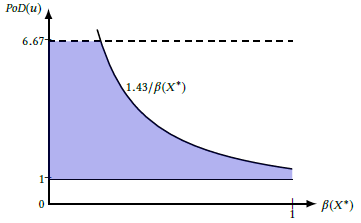
\includegraphics[scale=0.7]{figs/podbounds.png}
	\end{center}
	\caption{$\PoD$ vs disparity parameter for the HDB problem with current EIP quotas and ethnic proportions from Census 2010.\label{fig:PoDbeta}}
\end{wrapfigure}

\subsection{Experimental Analysis}\label{sec:experiments}
In this section, we present simulations of the \ASTC problem using recent, publicly available datasets: Singapore demographic and housing allocation statistics, and the Chicago public school admission data. 
We compare the welfare of three assignment mechanisms: unconstrained optimal (maximizing welfare while ignoring the diversity constraints), constrained optimal (finding the optimal allocation under diversity constraints), and one-shot lottery-based (running a lottery with diversity constraints, as is the case for the HDB mechanism).\footnote{We generated a uniformly random sequence over agents and assigned to each an item for which it has the highest utility among unassigned items in blocks for which that agent's ethnicity quota had not been filled yet. We abstract away other complications of actual lottery-based approaches used in our problem domains to focus on diversity constraints.} Conducting large-scale surveys to elicit agent preferences over items was beyond the scope of this work, so we simulated utilities based on reasonable models for both problems. We solved both the unconstrained and constrained social welfare maximizations using the Gurobi Optimizer. We refer the reader to \url{https://git.io/fNhhm} for full implementation details. 
\begin{wrapfigure}[25]{R}{0.35\textwidth}
	\vspace{-12pt}
	\begin{center}
		\begin{tabular}[t]{c}
			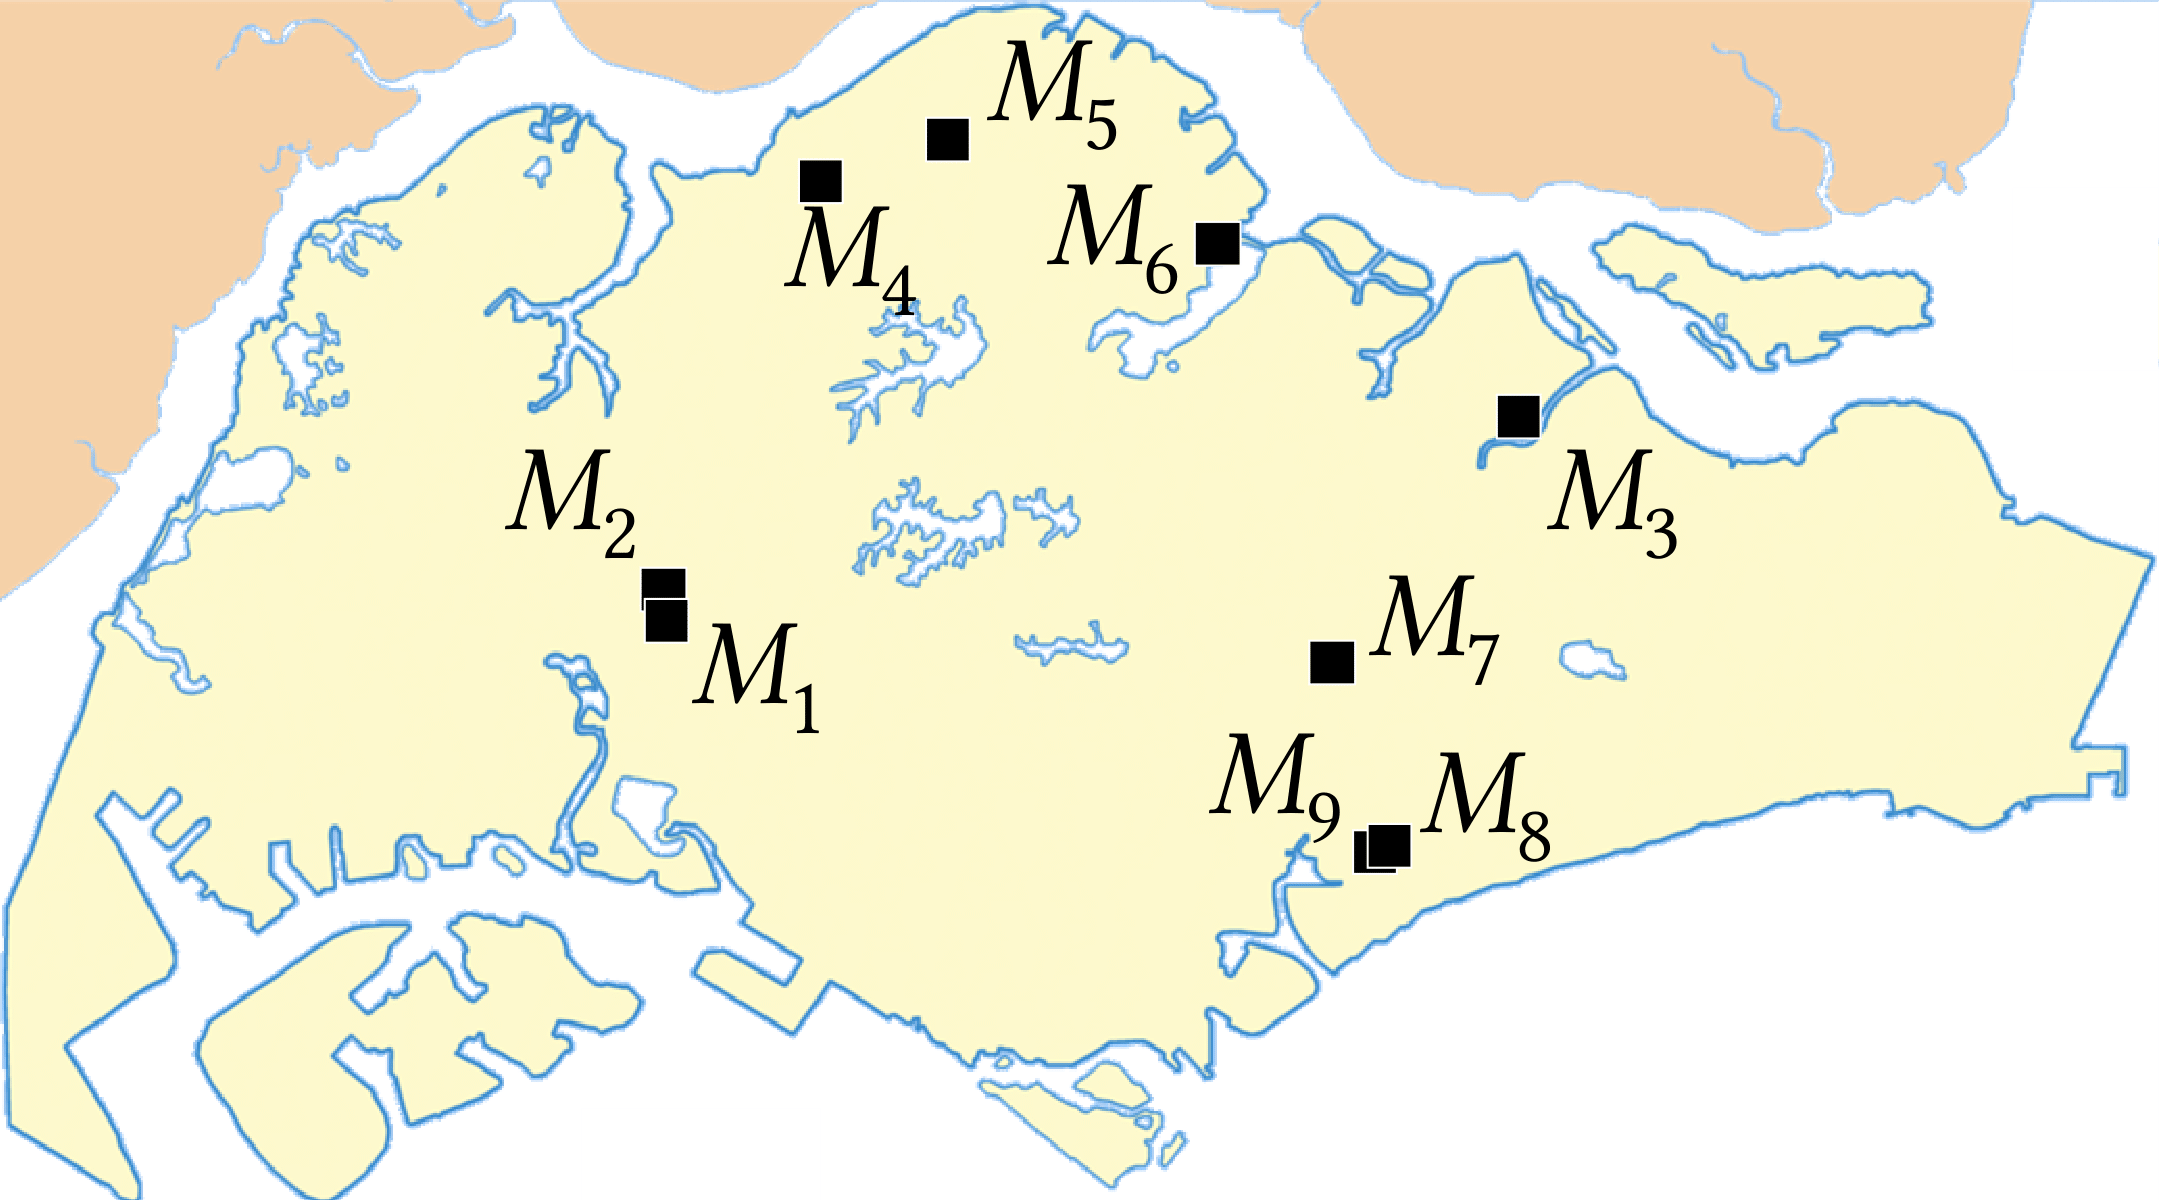
\includegraphics[scale=0.057]{figs/Map01Final081.png}\\ 
			(a)\\
			\\
			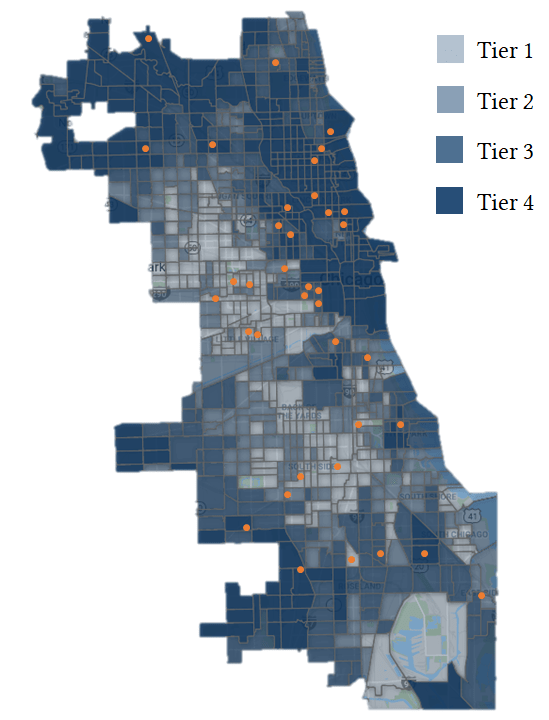
\includegraphics[scale=0.19]{figs/Chicago_Tier_School.png}\\
			(b)
		\end{tabular}
	\end{center}
	\caption{(a) Singapore public housing block locations. (b) Tier statuses of Chicago census tracts and magnet school locations (orange dots). \label{figMap}}
\end{wrapfigure}
\paragraph{The Singapore Public Housing Allocation Problem.} 
We collected data on the locations and numbers of flats of recent HDB housing development projects advertised over the second and third quarters of 2017.\footnote{\url{http://www.hdb.gov.sg/cs/infoweb/residential/buying-a-flat/new/bto-sbf}} 
Each development constitutes a block in our simulations, for a total of $m = 1350$ flats partitioned into $l = 9$ blocks $M_1, \ldots, M_9$ (Figure \ref{figMap}(a)), consisting of 128, 162, 156, 249, 108, 94, 104, 190, 159 flats respectively. There are pre-specified \emph{categories} of flats, viz. 2-room flexi, 3-room, 4-room, and 5-room; our data set includes lower and upper bounds, $\LB(t,q)$ and $\UB(t,q)$ respectively, on the monthly cost (loan) for a flat of category $t$ in block $M_q$ for every $t$ and $q$.
We simulate $2$ pools of $n$ applicants whose ethnic composition follows the 2010 Singapore census report \cite{Sing2010}, as shown in Table~\ref{SGtable}.
\begin{wraptable}{O}{0.3\textwidth}
	\begin{tabular}{|c|c|c|c|}
		\hline
		$n$ & $|N_1|$& $|N_2|$ & $|N_3|$ \\ \hline
		$1350$ & $1000$ & $180$ & $170$\\
		$3000$ & $2223$ & $402$ & $375$\\ \hline
	\end{tabular}
\caption{$\#$applicants (types $1$, $2$, and $3$ are Chinese, Malay, Indian/Others respectively)\label{SGtable}}
\end{wraptable}
From the same census report, we collected the average salary $S(p)$ of each ethnicity group $p \in [k]$, given in Singapore dollars: $S(1) = S\$7,326$, $S(2)=S\$4,575$ and $S(3) = S\$7,664$. 
From publicly available data\footnote{\url{https://data.gov.sg/dataset/master-plan-2014-planning-area-boundary-web}} on Singapore's Master Plan 2014,\footnote{\url{https://www.ura.gov.sg/Corporate/Planning/Master-Plan/}} we glean the locations of the geographic centers of the $55$ planning areas that Singapore is divided into; we also obtained the population sizes of the three ethnicity groups under consideration in each planning area from the General Household Survey 2015 data available from the Department of Statistics, Singapore.\footnote{\url{https://www.singstat.gov.sg/publications/ghs/ghs2015content}}
Our block capacities follow latest HDB block quotas~\cite{deng2013publichousing}: $\alpha_{1q} = 0.87, \alpha_{2q} = 0.25$, $\alpha_{3q} = 0.15$ for every block $M_q$. 

We simulate $4$ utility models; each has one parameter that does not come from the data: \textbf{(i) {\em Distance-based} ($\Dist(\sigma^2)$)}: Each agent $i \in N$ has a preferred geographic location $\vec a_i \in \R^2$ (chosen uniformly at random within the physical landmass of Singapore) that she would like to live as close as possible to (say, the location of her parents' apartment, workplace, or preferred school). For every block $M_q$, we generate the utility of that agent $i$ for apartment $j \in M_q$ by first drawing a sample from the normal distribution $\mathcal{N}(1/ d(\vec a_i,\loc(M_q)),\sigma^2)$, where $\loc(M_q) \in \R^2$ is the geographical location of block $M_q$ and $d(\cdot,\cdot)$ represents Euclidean distance, and then renormalizing to make the sum of utilities of each agent for all apartments in $M$ equal to 1. \textbf{(ii) {\em Type-based} ($\Ethn(\sigma^2)$)}: We assume that all agents of the same type (i.e., ethnic group) have the same preferred location (i.e.,  $\forall p \in [k], \forall i,i' \in N_p, \vec a_i = \vec a_{i'}$); the rest is similar to the above distance-based model. \textbf{(iii) {\em Project approval-based} ($\Proj(\rho)$)}: We construct, for each type, a categorical distribution over the $55$ planning areas of Singapore, the probability of each area being proportional to the fraction of the sub-population of that type living in that area; for each agent $i$, we sample a preferred planning area from the above distribution corresponding to $i$'s type; if a project $M_q$ is within a radius $\rho$ of the geographic center of agent $i$'s preferred planning area, then $i$ approves of the project i.e., $u(i,j) = 1$ $\forall j \in M_q$, else $i$ disapproves of the project i.e., $u(i,j) = 0$ $\forall j \in M_q$. \textbf{(iv) {\em Price-based} ($\Price(\sigma^2)$)}: Each agent $i \in N_p$ has a salary $s_i$ that is generated according to the normal distribution $\mathcal{N}(S(p),\sigma^2)$. Each flat $j \in M_q$ of category $t$ has a monthly cost $p_j$ chosen uniformly in $[\mathit{LB}(t,q), \mathit{UB}(t,q)]$. 
The utility that agent $i$ derives from flat $j$ is then defined by $u(i,j)= 1/(p_j - \frac{s_i}{3})^2$, assuming that agent $i$ is willing to pay one-third of her monthly salary on mortgage installments;\footnote{Inspired by the Singapore Central Provident Fund Board-endorsed ``3-3-5 rule", as of 21 Sep 2017.} the rationale for the utility formula is that a high cost relative to the budget makes flats unaffordable, while a much lower cost indicates unsatisfactory quality, making the agent unhappy in both scenarios. 

For each of our treatments (Figures~\ref{figTests1}--\ref{figTests3}), we plot the realized $\PoD(u)$ (hatched bar), the theoretical upper bound on $\PoD(u)$ as per Theorem~\ref{thm_parampod} (dark gray bar), and the relative loss of the HDB lottery mechanism (i.e., the ratio of $\OPT(u)$ to the total utility of the assignment produced by the lottery mechanism) averaged over 100 agent permutations (light gray bar) against the values of the corresponding model parameters ($\sigma^2$ or $\rho$). 
In order to compare $\Dist(\sigma^2)$ with $\Ethn(\sigma^2)$, we vary both $\sigma^2$ in $\{1,5,10\}$ and $n$ in $\{1350, 3000\}$; 
the results reported in Figures~\ref{figTests1} are on average performance over $100$ randomly generated instances. 
Our first observation is that, in all our experiments, $\Dist(\sigma^2)$ exhibits virtually no utility loss due to the imposition of type-block constraints (see the hatched bars in Figures~\ref{figTests1}(a)). 
This is because utilities in $\Dist(\sigma^2)$ are independent of ethnicity, resulting in a very low value for the inter-type disparity parameter $\beta$ (indicated by the dark gray bars) --- in fact, for any utility model where utilities are independent of ethnicity, the expected value of the disparity parameter is $1$. 
For the $\Ethn(\sigma^2)$ model-based utilities, the disparity parameter is somewhat higher (utilities do strongly depend on ethnicity), resulting in a higher $\PoD(u)$ (see the hatched bars in Figures~\ref{figTests1}(b)). 
\begin{figure}[t]
	\begin{center}
		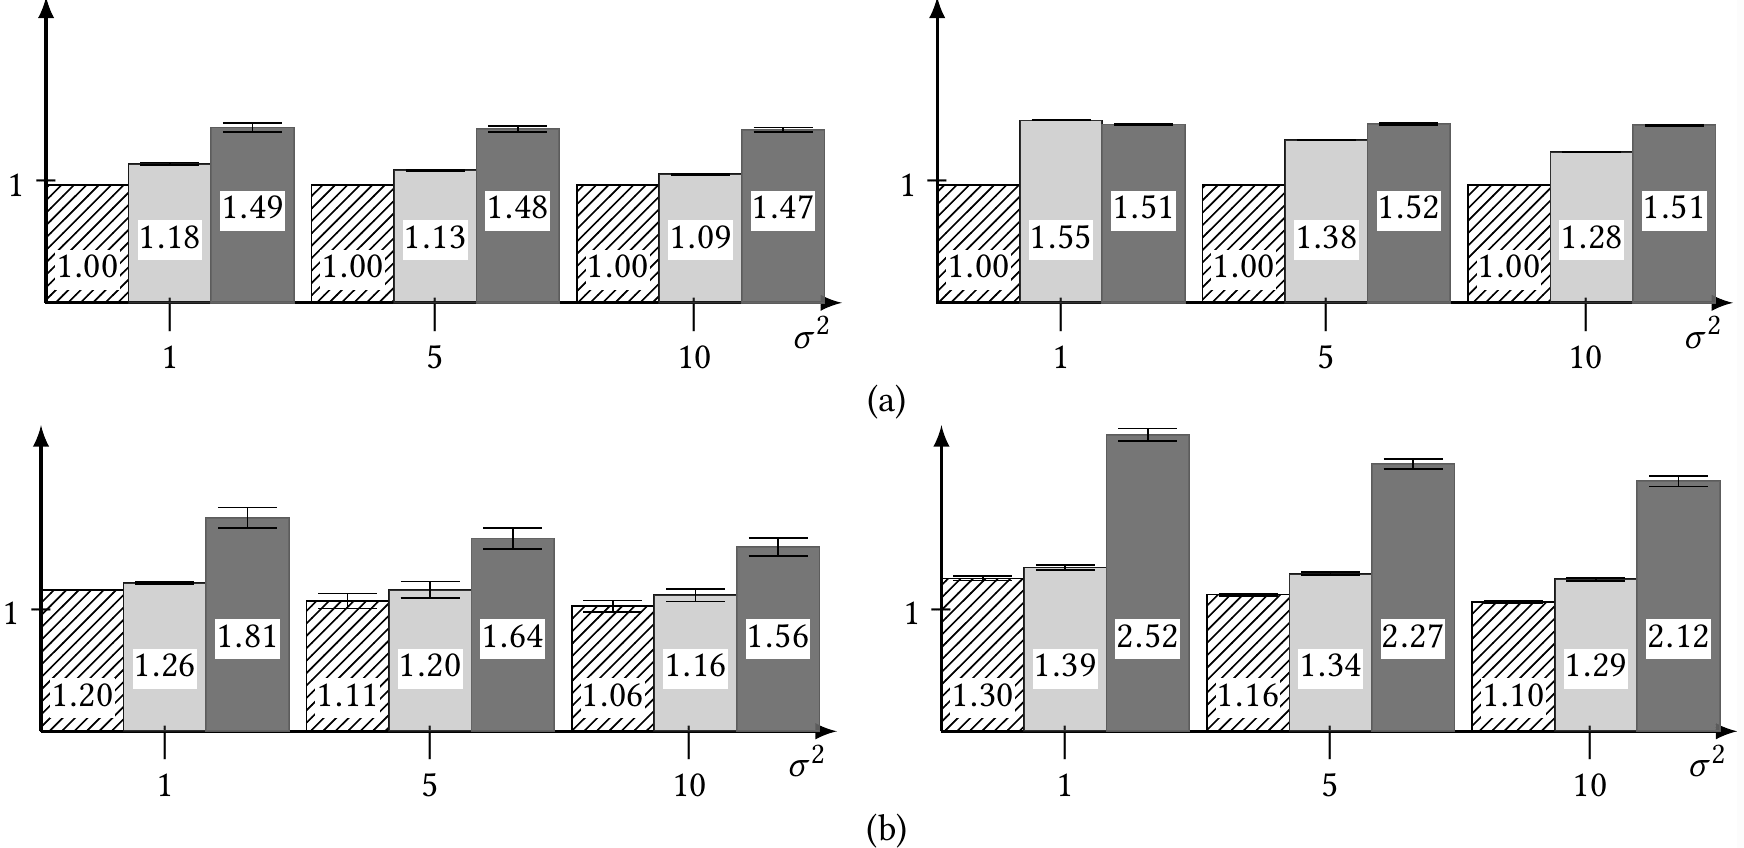
\includegraphics[scale=0.21]{figs/sing1.png}
	\end{center}
	\caption{Averaged utility losses for (a) $\Dist(\sigma^2)$ and (b) $\Ethn(\sigma^2)$ with $n = m = 1350$ (left) and $n = 3000$, $m = 1350$ (right). \label{figTests1}}
\end{figure}
Despite making no attempt to optimize social welfare under type-block constraints, the HDB lottery mechanism does surprisingly well when the number of agents equals the number of apartments (see the light gray bars in the left part of Figure~\ref{figTests1}), extracting at least $84\%$ of the optimal unconstrained welfare under the $\Dist(\sigma^2)$ utility model, and at least $79\%$ of the social welfare under the $\Ethn(\sigma^2)$ model. 
However, the lottery-induced welfare is negatively impacted by the number of agents (see the light gray bars in the right part of Figure~\ref{figTests1}); 
for instance, it only extracts $65\%$ of the optimal unconstrained welfare under $\Dist(1)$ with $n=3000$ and, in fact, the lottery-induced welfare loss for this treatment even exceeds the theoretical upper bound on the price of diversity.

For $\Proj(\rho)$, we use the fact that one degree of latitude or longitude at the location of Singapore corresponds to roughly 111 km to compute distances; we vary $\rho$ in $\{5,7.5,10\}$ (in km). The results averaged over 100 runs are provided in Figure~\ref{fig:ProjApprov}. In all instances, $\PoD(u)$ is almost one and the lottery-induced welfare is also nearly as good, achieving at least $87\%$ of the unconstrained optimum for $1350$ agents and practically $100\%$ for $3000$ agents; the disparity parameter is also consistently close to its ideal value of $1$, keeping the upper bound at around $1.45$ regardless of the radius. Thus, this can be considered an example of a utility model for which the lottery mechanism virtually implements a constrained optimal allocation for a wide range of model parameters.
\begin{figure}[t]
	\begin{center}
		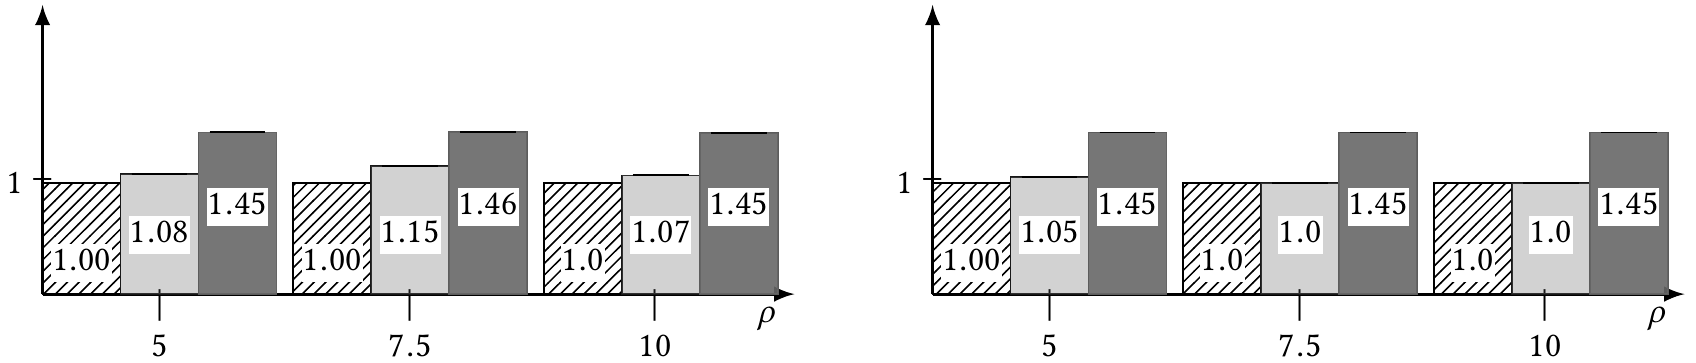
\includegraphics[scale=0.21]{figs/sing2.png}
	\end{center}
	\caption{Averaged utility losses for $\Proj(\rho)$ with $n = m = 1350$ (left) and $n = 3000$, $m = 1350$ (right). \label{fig:ProjApprov}}
\end{figure}
Finally, for $\Price(\sigma^2)$, we  vary $\sigma^2$ in $\{0,10,50\}$; the results obtained by averaging over 100 runs are given in Figure~\ref{figTests3}.
While the price of diversity is practically equal to one in all instances, the welfare loss observed with the lottery mechanism drastically increases with $\sigma^2$ (recall that agents from the same ethnicity group have identical preferences when $\sigma^2 = 0$): for instance, for $1350$ agents, it extracts $98\%$ of the optimal unconstrained welfare under $\Price(0)$ while it only extracts $35\%$ of this value under $\Price(50)$. 
%Moreover, for $\Price(50)$, %we found problem instances in which the the welfare loss induced by the lottery mechanism exceeds the corresponding theoretical upper bound on $\PoD(u)$.
%we observe that the welfare loss induced by the lottery mechanism exceeds the theoretical upper bound on $\PoD(u)$ in some instances with $1350$ agents. %(but this effect appears to be mitigated by a larger number of agents in our experiments). 
These numerical tests show that utility models exist for which the lottery mechanism may perform poorly compared to the optimal constrained allocation mechanism, even in allocation problems with a very low price of diversity.
\begin{figure}[t]
	\begin{center}
		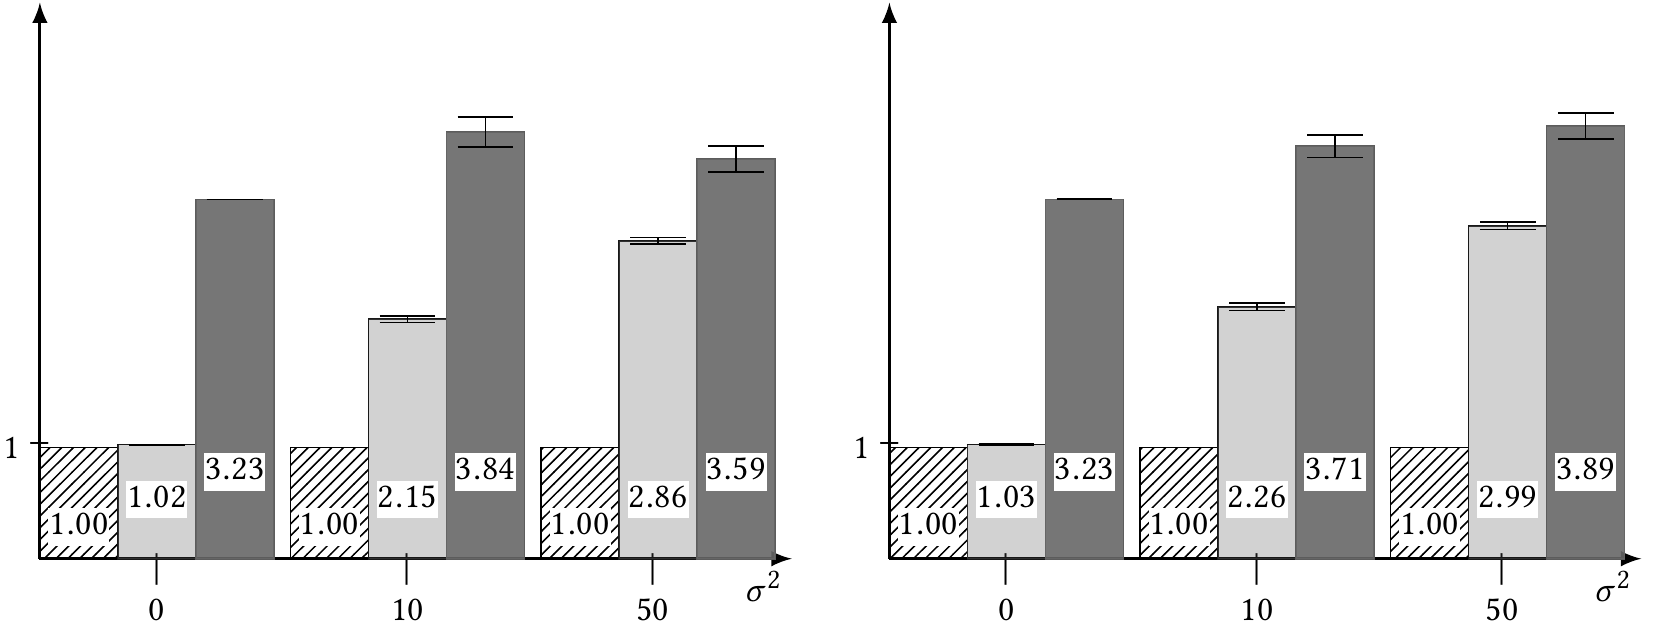
\includegraphics[scale=0.21]{figs/sing3.png}
	\end{center}
	\caption{Averaged utility losses for $\Price(\sigma^2)$ with $n = m = 1350$ (left) and $n = 3000$, $m = 1350$ (right). \label{figTests3}}
\end{figure}
\paragraph{Chicago Public School Admissions.} Chicago Public Schools (CPS) is one of the largest school districts in the U.S.A.,\footnote{\url{http://www.cps.edu/About_CPS/At-a-glance/Pages/Stats_and_facts.aspx}} overseeing more than 600 schools of various types.\footnote{\url{http://cpstiers.opencityapps.org/about.html}} The application and selection processes for these schools involve a number of computerized lotteries, 
with a significant number of entry-level seats in magnet and selective enrollment schools being filled by lotteries based on a \emph{tier system} based on the family \emph{socio-economic status} (SES) as part of a social integration policy. 
The city computes a multi-factor, composite SES score for each of the census tracts that Chicago is divided into, and places each tract in one of four tiers based on its score in such a way that each tier contains (roughly) a quarter of school-aged children. 
The tier of a child is determined by their residential address. 
Of the seats in each school earmarked for a \emph{citywide SES lottery} or \emph{general lottery}, an equal number is allocated to each tier, and there is an upper limit on the number of schools that a child may apply to (see \cite{schools2017chicago,quick2016chicago}). 
We apply our setup to a simplified version of the CPS student-seat allocation scenario.

We collected data from the Chicago Public Schools website\footnote{\url{http://cps.edu/Pages/home.aspx}} on the locations of magnet schools in Chicago (which use a lottery mechanism to select students), as well as the total number of students enrolled in these schools in 2018, which we divided by $9$ to obtain the approximate number of first-graders (there are nine grades in total). 
This leads us to instances with $l=37$ blocks (schools) and $m = 2261$ items (available seats) in total. 
In this school admission problem, students are partitioned into $k=4$ types, viz. Tiers 1, 2, 3 and 4, depending on their residence (see Figure \ref{figMap}(b)\footnote{Based on data from \url{http://cpstiers.opencityapps.org/} and \url{http://cps.edu/ScriptLibrary/Map-SchoolLocator/index.html}.}). In our experiments, we simulate $2$ pools of $n$ students where the type composition follows the real-world proportion, as shown in Table~\ref{Chictable}. Our type-block capacities are $\lambda_{pq} = 0.25 |M_q|$ for every pair $(p,q)$. For our student-seat utility simulations, we use the distance-based utility model $\Dist(\sigma^2)$ we introduced in the housing domain, with the following important modifications: 
we choose the preferred location of a student uniformly at random from the collection of census tracts (polygons) belonging to her tier (see Figure \ref{figMap}(b)), where the position of every polygon is approximated by taking the averaged coordinates of its extreme points; we reset each student's utility to $0$ for any school ranked $21$st or lower in the preference ordering induced by her utilities (since students are allowed to apply to at most 20 schools), and then renormalize the utilities.

\begin{wraptable}[9]{l}{0.36\textwidth}
\begin{tabular}{|c|c|c|c|c|}
	\hline
	$n$ & $|N_1|$& $|N_2|$& $|N_3|$ & $|N_4|$\\ \hline
	$2261$ & $613$ & $622$ & $533$ & $493$\\
	$5000$ & $1355$ & $1375$ & $1180$ & $1090$\\ \hline
\end{tabular}
\caption{$\#$students (type $p$ is Tier $p$ for each $p \in [4]$.)\label{Chictable}}
\end{wraptable}

In our experiments, we vary $\sigma^2$ in $\{0,10,50\}$, and report 100-run averages of the same measurements as in the Singapore-based simulations (Figure \ref{figTests4}). We observe that both the price of diversity (hatched) and the loss of the lottery mechanism (light gray bar) decrease as $\sigma^2$ increases, remaining well below the Theorem~\ref{thm_parampod} bound (dark gray). However, the lottery mechanism loss is quite high in all instances and, just as in the Singapore case, gets worse for a higher number of students. Our experiments suggest that the lottery mechanism is better suited to problems with an equal number of agents and items.

\begin{figure}[t]
	\begin{center}
		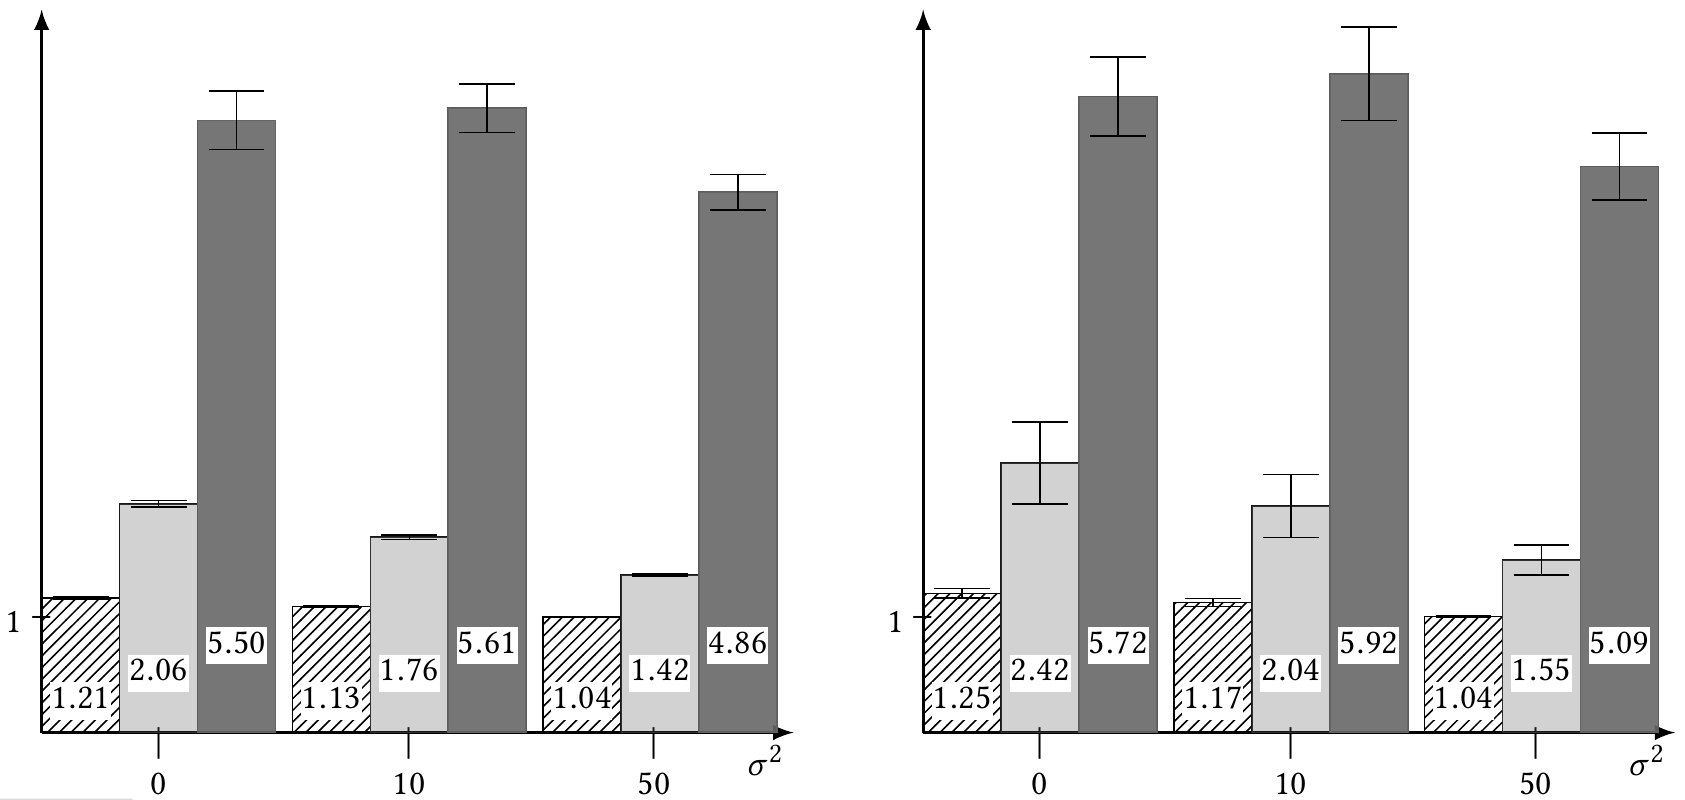
\includegraphics[scale=0.21]{figs/chicago.png}
	\end{center}
	\caption{Averaged utility losses for $\Dist(\sigma^2)$ with $n = m = 2261$ (left) and $n = 5000, m = 2261$ (right) in our Chicago-based simulations. \label{figTests4}}
\end{figure}

\section{Group Fairness in Allocation}\label{sec:grfair}
Up to this point, we have only explored the welfare loss due to capacity constraints; however, allocative efficiency is only one facet of group fairness. In some settings, groups might receive an overall worse outcome from the allocation mechanism, as compared to others. This is known in the fairness literature as {\em envy}. In this section, we explore how envy-freeness (i.e., having no agent group envy another's allocation) affects the allocation outcome.
We work with a model similar to that in Section~\ref{sec:assigntc} with two differences: (i) the items $M$ are not partitioned into blocks (or, equivalently, there is one block); (ii) we assume that for each agent $i \in N$ (resp. item $j \in M$), there is at least one item $j \in M$ (resp. agent $i \in N$) with $u(i,j)>0$. 
We adopt an alternative view of diversity-respecting assignment as a task of allocating bundles (i.e., disjoint subsets of $M$) to \emph{super-agents} (i.e., the types $N_1, \ldots, N_k$) in a manner that is both \emph{fair} and \emph{efficient} (see \cite{benabbou2019fairness} for further details and complete proofs). 

Each type $p$ is represented by a {\em super-agent}. We define $v_p(S)$, the \emph{valuation} of any super-agent $p \in [k]$ for any bundle of items $S \subseteq M$, as the maximum utilitarian social welfare of matching items in $S$ to agents of type $N_p$; $v_p(\cdot)$ is a monotonic, submodular set function (see \cite[Theorem 1]{benabbou2019fairness}). 
Moreover, our model does not satisfy the additive bundle-valuation assumption or the public goods assumption prevalent in most prior work (see e.g., \cite{caragiannis2016unreasonable,barman2018greedy,aleksandrov2018group,segal2018democratic} and references therein), necessitating novel solution techniques.
\begin{definition}[Allocation]\label{defn:alloc}
	An \emph{allocation} $\mathcal{A}$ is a collection of bundles $M^\mathcal{A}_1$,$ \cdots$, $M^\mathcal{A}_k$, such that $M^\mathcal{A}_1 \cup \ldots \cup M^\mathcal{A}_k \subseteq M$ and $M^\mathcal{A}_p \cap M^\mathcal{A}_q = \emptyset$ for all $p,q \in [k]$ with $p \neq q$, along with a maximum-$\USW$ matching between each type $N_p$ and its allocated bundle $M^\mathcal{A}_p$ for all $p \in [k]$, thereby inducing a unique $(N,M)$-matching $X^{\mathcal{A}} = (x^{\mathcal{A}}_{ij} )_{i \in N, j \in M}$.
\end{definition}
We call $M^\mathcal{A}_0 = M \backslash \cup_{p\in [k]} M^\mathcal{A}_p$ the set of \emph{withheld items} under allocation $\mathcal{A}$. In general, withholding items means that an allocation violates, by definition, the \emph{completeness} condition, a commonly used efficiency criterion. 
A type $p$'s \emph{marginal utility} for an item $j$ is the difference in $p$'s valuation of $S$ with and without item $j$: $\Delta_p(S;j) \triangleq v_p(S \cup \{j\}) - v_p(S)$ if $j \notin S$; $\Delta_p(S;j) \triangleq v_p(S) - v_p(S \backslash \{j\})$ if $j \in S$.
%\begin{align*}
%\Delta_p(S;j) \triangleq \begin{cases}
%v_p(S \cup \{j\}) - v_p(S)& \mbox{if }j \notin S\\ 
%v_p(S) - v_p(S \backslash \{j\})&\mbox{if }j \in S. 
%\end{cases}
%\end{align*}
We say that an item $j \in M^\mathcal{A}_p$ is \emph{unused} under $\mathcal{A}$ if it is either unassigned in the corresponding matching between $N_p$ and $M^\mathcal{A}_p$ or is assigned to an agent $i \in N_p$ such that $u(i,j)=0$. \emph{Cleaning} is the procedure of revoking all unused items from an allocation and putting them in the withheld set.
An item $j \in M$ is \emph{wasted} by an allocation $\mathcal{A}$ if it is either withheld (i.e., $j \in M^\mathcal{A}_0$) or allocated to a type $p$ and unused, although there is some other type $q$ with $\Delta_q(M^\mathcal{A}_q;j) > 0$. A {\em non-wasteful} allocation has no wasted items. Non-wastefulness is a reasonable efficiency concept in this setting; in fact, it turns out to be a relaxation (\cite[Lemma 1]{benabbou2019fairness}) of a popular efficiency criterion, \emph{Pareto optimality}: an allocation is Pareto optimal among types if the realized bundle-value of no type under this allocation can be strictly improved without strictly diminishing that of another.

We base our fairness criterion on the concept of \emph{envy}: a type $p$ envies a type $q$ if $v_p(M^\mathcal{A}_p) < v_p(M^\mathcal{A}_q)$; $p$ envies $q$ up to $\nu$ items, $\nu \in [|M^\mathcal{A}_q|]$, if there is a subset $C \subseteq M^\mathcal{A}_q$ of size $|C|=\nu$ such that $v_p(M^\mathcal{A}_p) \ge v_p(M^\mathcal{A}_q \backslash C)$ and, for every subset $C' \subseteq M^\mathcal{A}_q$ with $|C'| < \nu$, $v_p(M^\mathcal{A}_p) < v_p(M^\mathcal{A}_q \backslash C')$. Ideally, we want no type to envy another but such an allocation may not exist; a relaxation that always exists is the following:
\begin{definition}[Envy-freeness up to one item \cite{budish2011combinatorial}]\label{defn:tef1}
	Allocation $\mathcal{A}$ is \emph{envy-free up to one item} (EF1) among types if for any two types $p,q \in [k]$, $p$ either does not envy $q$ or envies $q$ up to one item i.e., there exists an item $j \in M^\mathcal{A}_q$ such that $v_p(M^\mathcal{A}_p) \ge v_p(M^\mathcal{A}_q \backslash \{j\})$.
\end{definition}
We want our allocation to be not just EF1 among types (thereby respecting diversity) but also efficient in one of the ways discussed above. Our first result in this vein applies to the \emph{binary utility model}: $u(i,j) \in \{0,1\}$, $\forall i \in N$, $\forall j \in M$.
This captures scenarios where each agent either approves or disapproves of an item but does not distinguish among its approved items.  %There exists prior work on fair allocation algorithms producing allocations with binary item utilities \cite{barman2018greedy} but most assume additive bundle valuations. 
Moreover, in formal conversations with stakeholders, we have found that a binary utility model is likely consistent with how agents value items in many real-world situations, e.g., in housing markets, a potential buyer might want a flat of a particular category only (such as a 3BHK within a 5-km radius of her workplace), being indifferent among flats of the same category.
\begin{theorem}\label{thm:bin_all}
	For any problem instance with a binary utility model, Algorithm~\ref{alg_bin} computes in $\poly(n,m)$ time an EF1 allocation that also maximizes the utilitarian social welfare of the induced $(N,M)$-matching.
\end{theorem}
\begin{algorithm}
	\DontPrintSemicolon
	\caption{Maximum-size Matching with Envy-Induced Transfers}\label{alg_bin}
	
	Compute a maximum-size matching of bipartite graph $(N,M)$ such that there is an edge between $i$ and $j$ iff $u(i,j)=1$, and clean the resulting allocation; designate the subset of items matched to agents in $N_p$ as type $p$'s allocated bundle $M^\mathcal{A}_p$ $\forall p \in [k]$. \label{MM}\\						
	\textbf{/*Envy-Induced Transfers*/}\\
	\While{there are two types $p,q$ such that $p$ envies $q$ up to more than $1$ item.}
	{
		Find item $j' \in M^\mathcal{A}_q$ such that $\Delta_p(M^\mathcal{A}_p;j')>0$.\\
		$M^\mathcal{A}_q \leftarrow M^\mathcal{A}_q \backslash \{j'\}$; $M^\mathcal{A}_p \leftarrow M^\mathcal{A}_p \cup \{j'\}$.\\
		Compute a maximum-size $(N_p,M_p)$-matching.
	}			
\end{algorithm}
It is easy to see that optimal utilitarian social welfare automatically implies Pareto optimality among types, and hence non-wastefulness. Thus, Algorithm~\ref{alg_bin} solves the fair and efficient allocation problem for binary utilities.

For more general utilities in $\R_+$, an algorithm that guarantees a similarly fair and efficient allocation remains elusive. 
However, we note that it is possible to obtain a type-complete TEF1 allocation in polynomial time by a natural extension (called {\bf L} hereafter) of the algorithm due to Lipton et al.~\cite{lipton2004approximately}: iterate over the items $j \in M$, giving item $j$ to a type, say $p$, that is currently not envied by any other type for its current bundle $M_p$; compute an optimal matching with the augmented bundle $M_p \cup \{j\}$; construct the \emph{envy graph} where there is a directed edge from a type $q$ to a type $r$ whenever $q$ envies $r$ and eliminate any cycle in this graph by transferring  the bundle of every type on this cycle to its predecessor on this cycle (to ensure that there is an unenvied type in each iteration), followed by re-matching within each such type. 
Although no item is withheld, it is possible for the final allocation to be wasteful: an item may be allocated to a type which has zero marginal utility for it or may \emph{become} unassigned after a bundle is transferred between types. 



One heuristic that could reduce waste is the following: %instead of giving an item to an \emph{arbitrary} unenvied type in each iteration, find 
in each iteration, find an item-type pair having the maximum marginal utility among all currently unenvied types and all unallocated items (breaking further ties uniformly at random, say), and allocate that item to that type. We call {\bf L}, augmented with this heuristic, {\bf H}. 
\begin{wraptable}[8]{l}[-3pt]{0.36\textwidth}
	\begin{tabular}{|c|c||c|c|}
		\cline{3-4}
		\multicolumn{2}{c}{}  & \multicolumn{2}{|c|}{$\%Waste$}\\ \hline 
		Data set & $\#$Items & {\bf L} & {\bf H}\\ \hline 
		\multirow{2}{*}{\textsc{Unequal}} & $50$ & $13\%$ & $0$ \\ \cline{2-4}
		& $100$ & $39\%$ & $0$ \\ \hline
		\multirow{2}{*}{\textsc{Equal}}  & $50$ & $0\%$ & $0$ \\ \cline{2-4}
		& $100$ & $0.005\%$ & $0$ \\ \hline
	\end{tabular}
\end{wraptable}
To test how this marginal utility maximization heuristic performs in practice, we experimentally compared procedures {\bf L} and {\bf H} using the percentage of items wasted averaged over runs, denoted by $\%Waste$, as our performance metric. We simulated two data sets with $n = 100$ agents partitioned into $k=3$ types: \textsc{Unequal} (ethnic proportions following Singapore 2010 census \cite{Sing2010}): $|N_1| = 74$, $|N_2| = 13$, $|N_3| = 13$; 
\textsc{Equal}: $|N_p| \approx n/k$ for all types $p \in [k]$. For each agent, we sampled $m$ numbers uniformly at random from $[0,1]$ and normalized them to generate utilities for all $m$ items, with $m \in \{50,100\}$. The results are shown in the adjoining table: the main observation is that {\bf H} produces \emph{zero} waste for \emph{all} experiments. Thus, augmenting {\bf L} with a simple heuristic produces a surprising improvement in performance over a wide range of problem parameters.   

\section{Discussion and future work}\label{sec:concl}
One of the extensions of the work presented here that we are currently pursuing is a rigorous analysis of the lottery mechanism with diversity quotas which we experimentally compared with our constrained optimization benchmark in Section~\ref{sec:experiments}. We are trying to assess whether certain lotteries are better than others in maintaining diverse but efficient outcomes in theory and in practice i.e., how the different parameters (the number of types, their respective percentage caps, sizes, and their utility structures) interact with the randomness of the draws to affect the welfare of the entire population as well as welfare-discrepancies among types. 

One other major direction we are investigating is an extension of/alternative to Algorithm~\ref{alg_bin} for arbitrary real-valued utilities. Several other possible approaches towards a tradeoff between fairness/diversity and efficiency are also worth exploring: diversity through the optimization of carefully constructed objective functions \cite{lang2016multi, ahmed2017diverse}; extensions of non-envy-based fairness concepts (group-wise egalitarian welfare, maximin shares \cite{barman2017approx,barman2018groupwise}, etc.) to our matching-based setting, and so on. 

\section*{Acknowledgments}\label{sec:acks}
Chakraborty and Zick are supported by Singapore NRF Fellowship R-252-000-750-733, and Benabbou by ANR project 14-CE24-0007-01-Cocorico-CoDec; a major part of the work was done when Benabbou was a post-doctoral research fellow at National University of Singapore (2017-18), supported by Singapore NRF Fellowship R-252-000-750-733. 
The authors would like to thank Xuan-Vinh Ho, Jakub Sliwinski (supported by MOE grant R-252-000-6255-133), and Edith Elkind as co-authors of publications on which this article is based, and Ayumi Igarashi for insightful discussions.
Thanks are also due to the anonymous reviewers of AAMAS 2018 and IJCAI 2019, and the attendees of COMSOC 2018 and FAMAS 2019 where parts of this work were presented. 

% ---- Bibliography ----
\begin{thebibliography}{10} 
	\itemsep=1pt 
	\begin{small}
		
		\bibitem{ahmed2017diverse} F.~Ahmed, J.~P.~Dickerson, and M.~Fuge. \newblock {Diverse Weighted Bipartite $b$-Matching.} \newblock {\em Proc. 26th IJCAI}, pp. 35--41, 2017.
		
		\bibitem{aleksandrov2018group} M.~Aleksandrov and T.~Walsh, Toby. \newblock Group envy freeness and group Pareto efficiency in fair division with indivisible items. \newblock {\em K{\"u}nstliche Intelligenz}, pp. 57--72, 2018.
		
		\bibitem{barman2017approx} S.~Barman and S.~K.~Krishnamurthy. \newblock Approximation Algorithms for Maximin Fair Division. \newblock {\em Proc. 18th EC}, pp. 647--664, 2017.
	
		\bibitem{barman2017finding} S.~Barman, S.~K.~Krishnamurthy, and R.~Vaish. \newblock Finding Fair and Efficient Allocations. \newblock {\em Proc. 19th EC}, pp. 557-574, 2018.
	
		\bibitem{barman2018greedy} S.~Barman, S.~K.~Krishnamurthy, R.~Vaish. \newblock Greedy algorithms for maximizing {N}ash social welfare. \newblock {\em Proc. 17th AAMAS}, pp. 7--13, 2018.
	
		\bibitem{barman2018groupwise} S.~Barman, A.~Biswas, S.~K.~Krishnamurthy, and Y.~Narahari. \newblock Groupwise maximin fair allocation of indivisible goods. \newblock {\em Proc. 32nd AAAI}, pp. 917--924, 2018.
	
		\bibitem{benabbou2017diversity} N.~Benabbou, M.~Chakraborty, X.~V.~Ho, J.~Sliwinski, and Y.~Zick. \newblock {Diversity Constraints in Public Housing Allocation.} \newblock {\em Proc. 17th AAMAS}, pp. 973--981, 2018.
	
		\bibitem{benabbou2019fairness} N.~Benabbou, M.~Chakraborty, E.~Elkind, and Y.~Zick. \newblock Fairness Towards Groups of Agents in the Allocation of Indivisible Items \newblock {\em Accepted to 28th IJCAI}, 2019.
	
		\bibitem{bouveret2016fair} S.~Bouveret, Y.~Chevaleyre, and N.~Maudet. \newblock {Fair Allocation of Indivisible Goods.} \newblock {\em Handbook of Computational Social Choice}, ed. F.~Brandt, V.~Conitzer, U.~Endriss, J.~Lang, and A.~D.~Procaccia, ch. 12, pp. 284--310, {Cambridge University Press}, 2016.
	
		\bibitem{bredereck2018multiwinner} R.~Bredereck, P.~Faliszewski, A.~Igarashi, M.~Lackner, and P.~Skowron. \newblock Multiwinner Elections with Diversity Constraints. \newblock {\em Proc. 32nd AAAI}, pp. 933--940, 2018.
	
		\bibitem{budish2011combinatorial} E.~Budish \newblock The combinatorial assignment problem: Approximate competitive equilibrium from equal incomes. \newblock {\em Journal of Political Economy}, University of Chicago Press, Vol. 119, No. 6, pp. 1061--1103, 2011.
	
		\bibitem{caragiannis2016unreasonable} I.~Caragiannis, D.~Kurokawa, H.~Moulin, A.~D.~Procaccia, N.~Shah, J.~Wang. \newblock The unreasonable fairness of maximum Nash welfare. \newblock {\em Proc. 17th EC}, pp. 305--322, 2016.
	
		\bibitem{chua1991race} B.~Chua. \newblock {Race relations and public housing policy in Singapore.} \newblock {\em {Journal of Architectural and Planning Research}}, pp. 343--354, 1991.
	
		\bibitem{deng2013publichousing} Y.~Deng, T.~F.~Sing, and C.~Ren \newblock {The story of Singapore's public housing: From a nation of home-seekers to a nation of homeowners.} \newblock {\em The Future of Public Housing: Ongoing Trends in the East and the West}, ed. J.~Chen, M.~Stephens, and Y.~Man, ch. 7, pp. 103--121, Springer, 2013. ISBN 978-3-642-41621-7.
	
		\bibitem{fain2016core} B.~Fain, A.~Goel, and K.~Munagala. \newblock {The core of the participatory budgeting problem.} \newblock {\em Proc. 12th WINE}, pp. 384--399, 2016.
	
		\bibitem{fragiadakis2017improving} D.~Fragiadakis and P.~Troyan. \newblock {Improving matching under hard distributional constraints.} \newblock {\em Theoretical Economics}, Wiley Online Library, Vol. 12, No. 2, pp. 863--908, 2017.
	
		\bibitem{HDB10PR} {Housing and Development Board, Singapore.} \newblock {Policy changes to support an inclusive and cohesive home [Press release]. 5 Mar 2010.} \newblock \url{http://www.nas.gov.sg/archivesonline/speeches/record-details/809e76bf-115d-11e3-83d5-0050568939ad.}
	
		\bibitem{HDB18keystats} {Housing and Development Board, Singapore.} \newblock {Annual Report 2016/2017: Key Statistics. 2017} \newblock \url{http://www10.hdb.gov.sg/ebook/AR2018/key-statistics.html}.
	
		\bibitem{kamada2015efficient} Y.~Kamada and F.~Kojima. \newblock Efficient matching under distributional constraints: Theory and applications. \newblock {\em American Economic Review}, Vol. 105, No. 1, pp. 67--99, 2015.
	
		\bibitem{kim2013singapore} S.~Y.~Phang and K.~Kim. \newblock {Singapore's Housing Policies: 1960-2013.} \newblock {\em {Frontiers in Development Policy: Innovative Development Case Studies}}, pp. 123--153, 2013.
	
		\bibitem{kuhn1955hungarian} H.~W.~Kuhn. \newblock {The Hungarian method for the assignment problem.} \newblock {\em Naval Research Logistics}, 2(1-2):83--97, 1955.
	
		\bibitem{kurokawa2016can} D.~Kurokawa, A.~D.~Procaccia, and J.~Wang. \newblock When can the maximin share guarantee be guaranteed? \newblock {\em Proc. 30th AAAI}, pp. 523--529, 2016.
	
		\bibitem{lang2016multi} J.~Lang and P.~K.~Skowron \newblock Multi-Attribute Proportional Representation. \newblock {\em Proc. 30th AAAI}, pp. 530--536, 2016.
	
		\bibitem{lipton2004approximately} R.~J.~Lipton, E.~Markakis, E.~Mossel, and A.~Saberi. \newblock {On approximately fair allocations of indivisible goods.} \newblock {\em Proc. 5th EC}, pp. 125--131, 2004.
	
		\bibitem{lovasz2009matching} L.~Lov{\'a}sz and M.~D.~Plummer. \newblock {Matching theory.} \newblock {\em {American Mathematical Society}}, Vol. 367, 2009. 
	
		\bibitem{munkres1957algo} J.~Munkres. \newblock Algorithms for the assignment and transportation problems. \newblock {\em Journal of SIAM}, Vol. 5, No. 1, pp. 32--38, 1957.
	
		\bibitem{Parl1989} {Parliament of Singapore.} \newblock {Better racial mix in HDB housing estates.} \newblock {Parliament Debates: Official Report. 16 Feb 1989. Vol. 52, cols. 650-668.}
	
		\bibitem{procaccia2014fair} A.~D.~Procaccia and J.~Wang. \newblock {Fair enough: Guaranteeing approximate maximin shares.} \newblock {\em Proc. 15th EC}, pp. 675--692, 2014.
	
		\bibitem{quick2016chicago} K.~Quick. \newblock Chicago Public Schools: Ensuring Diversity in Selective Enrollment and Magnet Schools. \newblock {\em The Century Foundation.}  \url{https://tcf.org/content/report/chicago-public-schools}, 14 Oct 2016.
	
		\bibitem{schools2017chicago} Chicago Public Schools \newblock Chicago Public Schools Policy Manual: Admissions Policy for Magnet, Selective Enrollment and Other Options For Knowledge Schools and Programs. \newblock Section 202.2. Board Report 17-0426-PO2. Available at \url{http://policy.cps.edu/Policies.aspx}, 26 Apr 2017.
	
		\bibitem{segal2018democratic} E.~Segal-Halevi and W.~Suksompong. \newblock Democratic Fair Allocation of Indivisible Goods. \newblock {\em Proc. 27th IJCAI}, pp. 482--488, 2018.
	
		\bibitem{sim2003public} L.~L.~Sim, S.~M.~Yu, and S.~S.~Han. \newblock {Public housing and ethnic integration in Singapore.} \newblock {\em {Habitat International}}, Vol. 27, No. 2, pp. 293--307, 2003.
	
		\bibitem{Sing2010} Department of Statistics, Singapore. \newblock {Singapore 2010 Census: Key Indicators of the Resident Population.} \newblock 2010.
	
		\bibitem{Sing2018} {Department of Statistics, Singapore.} \newblock {Singapore in Figures.} \newblock 2018.
	
		\bibitem{stoyanovich2018online} J.~Stoyanovich, K.~Yang, and H.V.~Jagadish. \newblock {Online set selection with fairness and diversity constraints.} \newblock {\em Proc. 21st EDBT}, pp. 241--252, 2018.
	
		\bibitem{USedu2017} {U.S. Department of Education, Office of Elementary and Secondary Education.} \newblock {Improving Outcomes for All Students: Strategies and Considerations to Increase Student Diversity.} \newblock Washington, D.C. \url{https://www.ed.gov/diversity-opportunity}, 19 Jan 2017.
	
		\bibitem{wong2014estimating} M.~Wong. \newblock {Estimating the distortionary effects of ethnic quotas in Singapore using housing transactions.} \newblock {\em Journal of Public Economics}, Vol. 115, pp. 131--145, 2014.
		
	\end{small} 
\end{thebibliography}

\end{document}